\title{CS-613 Machine Learning}
\author{
        Final Project\\
        Alec Peterson, Yifan Wang, Jenny Boroda\\
        Fall 2023
}
\date{}
\documentclass[11pt]{article}
\usepackage[margin=0.7in]{geometry}
\usepackage{graphicx}
\usepackage{float}
\usepackage{amsmath}
\usepackage{longtable}
\usepackage{hyperref}
\begin{document}
\maketitle
%\begin{abstract}
%\end{abstract}



\section{Abstract}
\label{S:1}
We explore machine learning approaches for predicting the success of telemarketing campaigns. Logistic regression, Naive Bayes, and random forest binary classification algorithms are evaluated on an imbalanced dataset of telemarketing campaigns for a Portuguese bank from 2008 - 2013 with $>$40,000 observations and 20 features. Algorithm hyperparameters were optimized through cross-validation and evaluating the area under the receiver operating characteristic curve (AUC). Optimal probability thresholds were selected based on greatest difference in True Positive Rate (TPR) and False Positive Rate (FPR) for each algorithm. A comparison of classification error metrics showed logistic regression and random forest were effective at separating classes with AUCs of 0.90 for the validation dataset compared to an AUC of 0.83 for Naive Bayes. Precision (0.28 - 0.30) and F1 metrics (0.41 - 0.45) indicate relatively high false positives and potential improvement in probability threshold selection, algorithmic optimization, feature engineering, and/or data collection.

\section{Introduction}
\label{S:2}
Several aspects of financial telemarketing campaigns can be improved and refined through machine learning approaches. Predictive models can be used to reduce and focus employee resources, reduce intrusiveness to customers, aid in client selection, and predict overall success of a telemarketing contact. Moro, Cortez, and Rita address these approaches extensively for telemarketing campaign for selling long-term deposits for Portuguese banks in "A data-driven approach to predict the success of bank telemarketing" $^1$. The authors explored logistic regression, decision trees, a neural network (multi-layer perceptron), and support vector machines classification algorithms to predict the success of obtaining a long-term deposit from clients (a binary outcome) with a dataset consisting of $>50,000$ phone contacts from May 2008 to June 2013. \\

While the original dataset consisted of 150 features related to bank client information, previous and current campaign metadata, interest rates, information and characteristics of the calling agent, and social/economic indicators, the authors refined these to 22 significant features. A version of this dataset with some of the relevant features is made available, though the exact features identified are not shared. The original 150 features are not made publicly available either, potentially due to privacy or other restrictions. Algorithm parameters were optimized through cross-validation approaches. \\

The primary evaluation metric of relevance used by Moro, Cortez, and Rita was area under the curve (AUC) generated from the true positive rate (TPR) vs. false positive rate (FPR), also known as the receiver operating characteristic (ROC) curve.  The AUCs ranged from 0.833 to 0.929, and are shown in the table below. The decision tree performed the worst with an AUC of 0.833, while the neural network was most performant, with an AUC of 0.929 

\begin{table}[h]
\centering
\caption{The primary evaluation metric}
\begin{tabular}{lllll}
\hline
\textbf{Metric}& \textbf{Logistic Regression}& \textbf{Decision Trees}& \textbf{Support Vector Machines}& \textbf{Neural Network}\\
\hline
AUC&0.900 &0.833&0.891&0.929\\
\hline
\label{tB}
\end{tabular}
\end{table}

Some authors have leveraged the dataset made available by Moro et al. and explored the use of more sophisticated neural networks $^2$ and {ensembles} $^3$ of tree-based predictors. We similarly seek to assess and subsequently detail the performance of a logistic regression classifier, as well as a probability-based Naïve Bayes classifier, and a random forest ensemble of decision trees using the dataset made available. These latter two algorithms were not explored by Moro et al.\\

\section{Evaluation}
\label{S:3}

\subsection{Pre-Processing}
\label{SS:3-1}

\subsubsection{Training Set, Validation Set, and Resampling}
 A training set (2/3 of observations) and validation set (1/3 of observations) were made by randomly shuffling then splitting the dataset while retaining the same proportion of class labels across the two sets.\\


The dataset class labels are imbalanced in that the positive class ("success" in telemarketing campaign outcome) represents only ~$11\%$ of entries in the dataset. The classification algorithms explored, especially logistic regression and random forest, were known to be sensitive to this imbalance and could give poor performance/generalization if not addressed during model training. A bootstrap resampling strategy was used in the training set, where the samples of the positive class labels were randomly drawn (allowing for repeated samples) and added to the training set so that the proportion of class labels were even between the positive and negative class label.

\subsubsection{Categorization of Numerical Features }
 
The data set shared by Moro et al. consists of the features described in Table 2. 

\begin{longtable}[hbt!]
{p{.01\textwidth}p{.12\textwidth}p{.10\textwidth}p{.20\textwidth}p{.45\textwidth}}%{lllll}
\caption{Dataset Features}\\
\hline
\textbf{\#}& \textbf{Feature}& \textbf{Type}& \textbf{Attribute Grouping}& \textbf{Description}\\
\hline
1&age&numeric&Bank Client Data&Age of client contacted\\
2&job &categorical& &Type of job (e.g. admin., unemployed, management, student, blue-collar, self-employed, etc.) \\
3&marital &categorical& &Marital status (married, divorced/widowed, single) \\
4&education &categorical& &Extent of education (primary, secondary, tertiary, unknown)  \\
5&default   &categorical& &If client has credit in default (yes, no) \\
6&housing &categorical& &If client has a housing loan (yes, no)\\
7&loan&categorical& &If client has a personal loan (yes, no) \\
8&contact &categorical&Last Contact in Current Campaign &Contact communication type (telephone, cellular, unknown)\\
9&day\_of\_week  &categorical& &Last contact day of the week\\
10&month   &categorical& &Last contact month of the year \\
11&duration &numeric& &Last contact duration, in seconds \\
12&campaign  &numeric&Previous Campaign &Number of contacts performed during this campaign for the client (including last contact) \\
13&pdays &numeric& &Number of days that have passed since client was last contacted from a previous campaign (-1 label for not previously contacted)\\
14&previous  &numeric& &Number of contacts prior to this campaign for the client \\
15&poutcome &categorical & &Outcome of previous marketing campaign (success, failure, unknown, other) \\
16&emp.var.rate &numeric &Social and Economic Indicators &Employment variation rate, with a quarterly frequency  \\
17&cons.price.idx  &numeric & &Monthly average consumer price index  \\
18&cons.conf.idx &numeric & &Monthly average consumer confidence index \\
19&eurobor3m  &numeric & &Daily three month Euribor rate  \\
20&nr\_employed   &numeric & &Quarterly average of the total number of employed citizens   \\
\label{tB}

\end{longtable}

The numerical features in this dataset were posited to be more effective at separating the classes if they were made into categorical features. For instance, the exact age of the bank client did not seem to matter as much as to which age group they belonged. This type of thinking is consistent with customer segmentation methods well-known to the general public.  \\

Similar assessments were made of the other numerical features, and categories were created based on exploratory data analysis (EDA) of the features and assessment of the proportion of class labels for the resulting categories. Categorization where one or more categories contained a larger proportion of “success” class labels, or vice versa, were sought. An objective categorization scheme could not be rigorously assessed as some features contained potentially limitless grouping options.  \\

From the EDA and assessment of weight-averaged entropy of a few different choices however, the chosen categories seemed appropriate and we feel alternate choices would not give significant improvements. Some numerical features were categorized into binary-valued features based on the mean of the training set. Features in the validation set used the mean of the corresponding feature in the training set for this transformation. \\

Table 3 below describes the categorization strategy made to the numerical features. The resulting dataset contained only categorical features. 

\begin{table}[hbt!]
\centering
\caption{Dataset Features}
\begin{tabular}{lll}
\hline
\textbf{\#}& \textbf{Feature}& \textbf{Categorization Scheme}\\
\hline
1&age&Split into categories: 17-30, 30-40, 40-60, 60-80, 80-100 years \\
11&duration &Converted seconds to minutes, then split into categories: 0-1, 1-2, 2-5, $>=5$ minutes  \\
12&campaign  &Split into categories: 0, 1, 2, 3-5, $>5$ contacts \\
13&pdays &Split into categories: -1-0, 0-180, 180-999 days since last contact \\
14&previous  &Split into categories: 0, 1, 2, 3-5, $>5$ prior contacts \\
16&emp.var.rate &Split into categories: -4 to -2, -2 to 0, 0 to -2 \\
17&cons.price.idx  &Split into binary category: 1 if $>=$ training set mean, else 0 \\
18&cons.conf.idx &Split into binary category: 1 if $>=$  training set mean, else 0 \\
19&eurobor3m  &Split into binary category: 1 if $>=$ training set mean, else 0\\
20&nr\_employed   &Split into binary category: 1 if $>=$ training set mean, else 0\\
\label{tB}
\end{tabular}
\end{table}

\subsubsection{Encoding}

The non-binary categorical features underwent one-hot encoding, creating a binary-valued (Boolean) column for each unique category present in the feature. For example, an age group category of “17-30 years” would be made into a column "is\_17-30 years". The resulting dataset combined these one-hot encoded features and existing binary features to give 81 features in total after pre-processing. 

\section{Algorithms}
\label{SS:4}

Logistic Regression, Naïve Bayes, and Random Forest binary classification algorithms were developed and optimized through 5-fold cross-validation and by ranking the resulting average area under the curve (AUC) across the 5 folds for each hyperparameter or hyperparameter combination (where applicable). This approach is described in more detail the following sections. The receiver operating characteristic curve (ROC) is used for performance evaluation for each of the classification models. ROC curves were prepared by plotting the True Positive Rate (TPR) against the False Positive Rate (FPR) as calculated by equations (1) and (2) at different classification thresholds (0 to 1, at intervals of 0.01). AUC was estimated using trapezoidal rule integration. \\

\begin{equation}
TPR = \frac{TP}{TP+FN}
\label{eqB}
\end{equation}
     \\

\begin{equation}
FPR = \frac{FP}{FP+TN}
\label{eqB}
\end{equation}

\indent  
The following classification metrics were also calculated for each of the algorithms tested:\\

\begin{equation}
Precision = \frac{TP}{TP+FP}
\label{eqB}
\end{equation}

\begin{equation}
Recall = \frac{TP}{TP+FN}
\label{eqB}
\end{equation}

\begin{equation}
F1 = 2 \frac{Precision * Recall}{Precision + Recall}
\label{eqB}
\end{equation}

\begin{equation}
Accuracy = \frac{TP+TN}{TP+TN+FP+FN}
\label{eqB}
\end{equation}
    

Where $TP$ = True Positives, $TN$ = True Negatives, $FP$ = False Positives, and $FN$ = False Negatives for binary classification.

\subsection{Logistic Regression}
\label{SS:4-1}

Logistic Regression (LR) is specifically designed for binary classification such as our outcome variable ("Success"/"Failure" of client giving long-term deposit). The class label probability for a logistic regression classifier is modeled by the following logistic sigmoid function: 
\begin{equation}
\label{eqA}
P(y=1|x)=g(x)=\frac{1}{1+e^{-(xw+b)}}
\end{equation}
where $w$ is a vector of weights corresponding to the features of the dataset, and $b$ is a bias weight. The implementation of logistic regression started with adding a bias feature to the dataset. Different sets of weights were produced through gradient descent, using a log-loss error function.  \\
 
Four different values were evaluated for the learning rate hyperparameter: 0.01, 0.1 1.0, 10.0.. The number of epochs used before finalizing the set of weights for each learning rate was 100. For each learning rate and fold as part of 5-fold cross-validation, ROC curves were generated and the areas under those curves calculated and then averaged. A learning rate of 1 gave the highest fold-average AUC of 0.90. \\

The ROC for the optimized Logistic regression classifier is shown below in Figure 1.
% \begin{figure}[hbt!]
\begin{figure}[H]
\centering
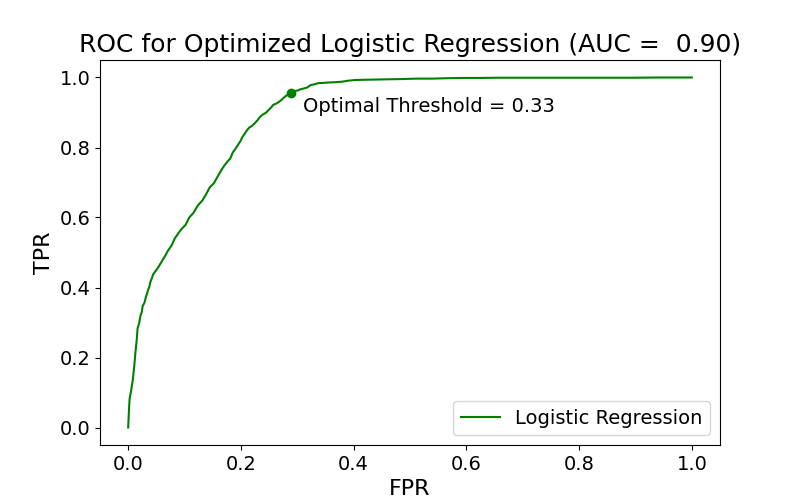
\includegraphics[width = 0.9\textwidth]{lr_roc.png} 
\caption{ The ROC for the optimized Logistic Regression classifier with an optimal probability threshold of 0.33, as determined by largest difference in TPR and FPR}
\label{ROC}
\end{figure}

This ROC curve represents the performance of the optimized logistic regression model in distinguishing between binary classes.  It plots the TPR against FPR across different probability thresholds, highlighting an optimal threshold at 0.33 based on the largest difference between TPR and FPR. This model suggests a good predictive capability with an AUC of 0.90, indicating a relatively high degree of separability for the class labels. 
 
Using a probability threshold of 0.33, the model can be further evaluated with the calculation of the classification metrics summarized in Table 4.  
   
\begin{table}[hbt!]
\centering
\caption{Classification Error Metrics for Optimized Logistic Regression}
\begin{tabular}{ll}
\hline
\textbf{Metric }& \textbf{Value }\\
\hline
AUC &0.90  \\
Precision &0.30   \\
Recall &0.96  \\
F1 &0.45 \\
Accuracy &0.74 \\
\label{tB}
\end{tabular}
\end{table}

With an AUC of 0.90, the model demonstrates a robust ability to differentiate between classes. However, a precision of 0.30 raises concerns about a substantial number of false positives, suggesting that while the model is adept at identifying true positives, as reflected in a high recall of 0.96, it often misclassifies negative cases as positive. The F1 score, which takes into account both precision and recall, stands at a moderate 0.45, indicating room for improvement in precision. Moreover, the accuracy of 0.74, while seemingly adequate, may be misleading, especially since the dataset is imbalanced. It does not reflect the disproportionate number of false positives that are inflating the model's performance metrics. \\
 
While logistic regression is straightforward and effective for establishing baseline performance, its applicability is constrained in complex or imbalanced datasets (hence the resampling approach previously described). This model tends to favor the majority class, leading to inaccurate predictions for the minority class—a significant disadvantage when precise classification is crucial. Furthermore, LR may fail when managing high-dimensional datasets that exhibit intricate feature interactions. An alternate Naïve Bayes classifier was considered as a complement to the baseline performance that the logistic regression algorithm offered.  

\subsection{Naïve Bayes Classifier}
\label{SS:4-2}

The Naïve Bayes (NB) classifier assumes the conditional probabilities of the features are independent and leverages Bayes rule to calculate the probability of a class label for a given observation. 
The posterior probability $P(y|x)$ is estimated from the class priors $P(y)$ and generative likelihoods $P(x|y)$ from the following equation. 

\begin{equation}
P(y|x)=\frac{P(y)P(x|y)}{P(x)}
\label{eqB}
\end{equation}

Posterior probabilities for the validation set are computed from the class priors and generative likelihoods in the training set. 
Cross-validation was not used for the Naïve Bayes classifier as there were no hyperparameters to optimize for this algorithm. 
Predicted targets were computed using the training set posterior probabilities.
The TPR and FPR were computed using the validation set and predicted target labels from the NB classifier.

The ROC for the optimized Naive Bayes classifier is shown below in Figure 2.\\
\begin{figure}[H]
\centering
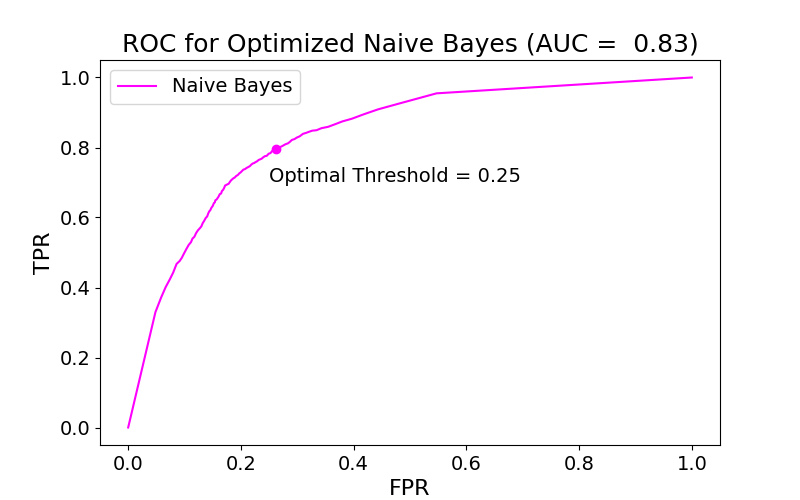
\includegraphics[width = 0.9\textwidth]{nb_roc.png} 
\caption{ The ROC for the optimized Naive Bayes classifier with an optimal probability threshold of 0.25, as determined by largest difference in TPR and FPR.}
\label{ROC}
\end{figure}

An optimal threshold of 0.25 was selected based on the greatest difference in TPR and FPR. The AUC and other classification error metrics are summarized in Table 5. 

\begin{table}[H]
% \begin{table}[hbt!]
\centering
\caption{Classification Error Metrics for Optimized Naive Bayes}
\begin{tabular}{ll}
\hline
\textbf{Metric }& \textbf{Value }\\
\hline
AUC &0.83  \\
Precision &0.28   \\
Recall &0.80  \\
F1 &0.41 \\
Accuracy &0.74 \\
\label{tB}
\end{tabular}
\end{table}
% \clearpage

While an AUC of 0.83 reflects comparable performance to the classifiers tested by Moro et al. and good separability in the class labels, the Precision, F1, and Accuracy are similar to LR for the probability threshold selected and show the model suffers from a relatively high number of false positives.

\subsection{Random Forest}
\label{SS:4-3}

A random forest is an ensemble of decision trees. To improve generalization of decision trees, multiple decision trees can be trained on a random subset of features and bootstrapped subsamples (random samples, with replacement) can be used in conjunction to provide a group estimate that is less prone to overfitting the training data. \\
 
The implementation of the random forest algorithm used an ensemble of binary decision trees, where the nodes of the tree require binary features to split the input data. The number of decision trees explored during optimization were 50, 100, and 300. \\
 
Bootstrapped samples using a subset of the data were used as input for each tree. The size of the subsets explored were $\sqrt{N}$, $N/2$, and $N$ where $N$ is the number of observations for the input dataset. For each split, only a certain number of features were considered. The values explored for this hyperparameter were $\sqrt{D}$, $\sqrt{D}/2$, and $2\sqrt{D}$ where $D$ is the total number of features.  \\
 
Splits were based on the feature with the lowest weight-averaged entropy. This is consistent with the ID3 algorithm for decision trees. Splits were performed until a maximum depth was reached, no more observations were present in the resulting split, only one class label was present in the resulting split, or no more features were available in the resulting split. The values explored for this maximum depth hyperparameter were 100, 500, 1000, and 3000. \\
 
The leaf nodes of each tree give a probability estimate for the positive class. Class label estimates could then be made based on the probability threshold. The grid of hyperparameters mentioned are summarized in Table 4 below. These combinations of hyperparameters were evaluated using 5-fold cross-validation and comparing the AUC corresponding to each set of parameters. \\
  

\begin{table} [h]
\centering
\caption{Combinations of hyperparameters}
%\begin{center}
\begin{tabular} {ll}
\hline 
\textbf{Hyperparameter }&\textbf{Values}\\
\hline
Sample Size for Tree & $\sqrt{N}$, 
N/2, 
Full \\
Number of Trees &50, 
100, 
300 \\
Maximum Depth  &100, 
500,
1000, 
3000 \\
Number of Features for Split &$\sqrt{D}$,
$\sqrt{D}/2$, 
$2*\sqrt{D}$ \\
\hline 
\end{tabular}
%\end{center}
\label{tA}
\end{table}
\begin{center}
    $N$ = number of observations, $D$ = number of features
\end{center}

From 5-fold cross-validation, the optimal random forest configuration used the full set of training observations for each decision tree, 300 trees, and $2\sqrt{D}$ for the $D$ features. The maximum depth did not seem to significantly affect the AUC, and all combinations of the aforementioned hyperparameters gave a fold-average AUC of 0.74 regardless of maximum depth.  \\
 
A combination of only half the set of training observations, 300 trees, $2\sqrt{D}$ for the $D$ features, and a maximum depth of 100 however gave a comparable AUC value of 0.73. From this and comparisons to other combinations of hyperparameter values, it appeared that the number of features trained for each tree had more of an impact than the number of trees (second most-important) or sample size (third most-important) used to train each tree. Due to the significantly lower compute resources required for this set of hyperparameters, it was used to evaluate performance on the validation set and compare against logistic regression and Naïve Bayes. \\

The ROC for the optimized random forest classifier is shown in Figure 3.



% \begin{figure}[hbt!]
\begin{figure}[H]
\centering
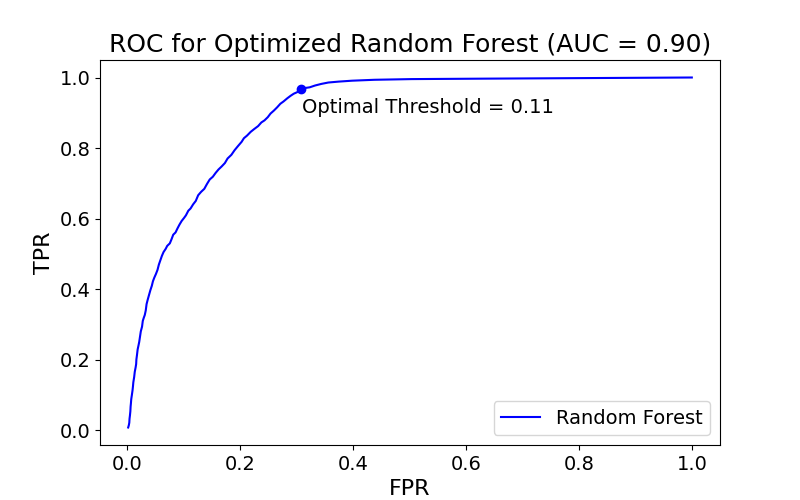
\includegraphics[width = 0.9\textwidth]{rf_roc.png} 
\caption{ ROC curve of validation set for random forest with 300 trees with each trained on half the set of training observations, 18 features ($2\sqrt{D}$ for $D = 81$), and a maximum depth of 100. ID3 algorithm used to split, based on weight-averaged entropy. }
\label{ROC}
\end{figure}

An optimal threshold was selected based on the greatest difference in TPR and FPR. This threshold is aligned with the positive class prior (positive class represents 11\% of data). The AUC and other error metrics are summarized in Table 7. 
% \begin{table}[hbt!]
\begin{table}[H]
\centering
\caption{Classification Error Metrics for Optimized Random Forest }
\begin{tabular}{ll}
\hline
\textbf{Metric }& \textbf{Value }\\
\hline
AUC &0.90  \\
Precision &0.29   \\
Recall &0.97  \\
F1 &0.44 \\
Accuracy &0.72 \\
\label{tB}
\end{tabular}
\end{table}

The random forest algorithm had a similar AUC and other metrics to logistic regression. A comparison of all the algorithms tested is subsequently described.


\section{Conclusion / Analysis}
\label{SS:5}

Figure 4 shows the overlaid ROC curves for the optimized algorithms tested.


\begin{figure}[hbt!]
\centering
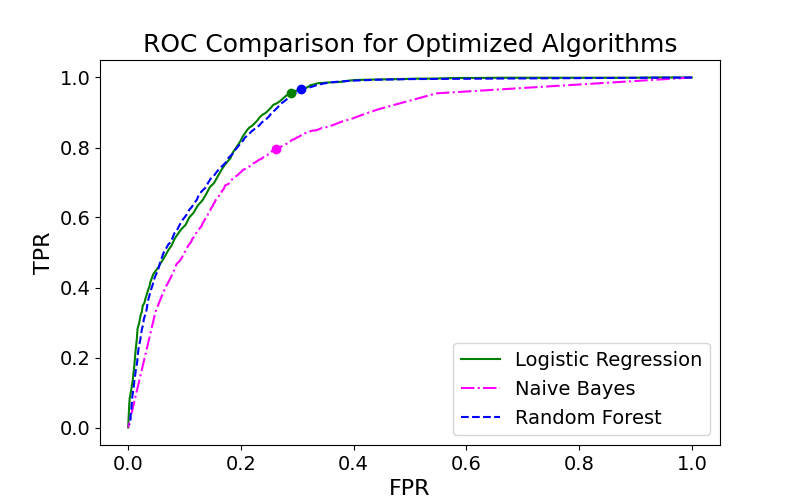
\includegraphics[width = 0.9\textwidth]{overlayed_roc.png} 
\caption{ ROC curves for optimized logistic regression, Naive Bayes, and random forest classifiers. Optimal probability thresholds, as determined by greatest difference in TPR and FPR, are highlighted.}
\label{ROC}
\end{figure}

The Naïve Bayes classifier shows the lowest performance of the three algorithms, as its ROC curve lies below that of the other two algorithms. The random forest and logistic regression performed essentially the same with their ROC curves overlapping closely. \\
 
Figure 5 shows AUC, Accuracy, Precision, Recall, and F1 score error metrics for the selected “optimal” thresholds giving the largest difference in TPR and FPR for a given optimized algorithm. \\
 
% \begin{figure}[hbt!]
\begin{figure}[H]
\centering
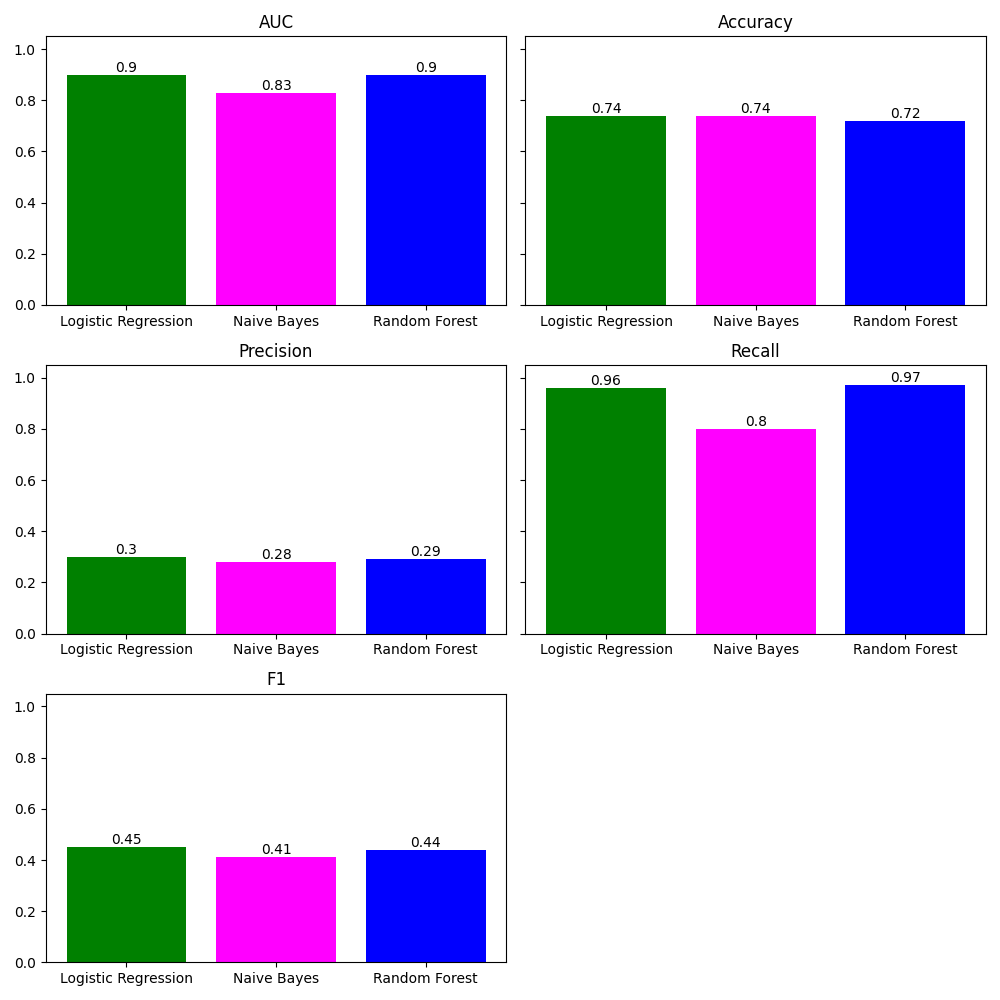
\includegraphics[width = 0.9\textwidth]{error_metrics_bar_charts.png} 
\caption{ Comparison of classification error metrics: AUC, Accuracy, Precision, Recall, and F1 for the logistic regression, Naive Bayes, and Random Forest classifiers}
\label{ROC}
\end{figure}


As suggested by the overlaid ROC curves in Figure 4, the AUC was lower for Naïve Bayes at 0.83 compared to the AUC of 0.90 for both logistic regression and random forest.  
Accuracy was comparable between the 3 algorithms at 72 to 74\%. Stakeholders for this classification model may prefer to select a probability threshold (or even sets of hyperparameters) that further prioritizes this value over AUC. This metric may be misleading though due to the imbalance of the class labels in the dataset. \\

The recall, equivalent to TPR, is relatively high for the models as the optimal threshold for each algorithm was selected to favor a high TPR while maintaining a low FPR. Of the “success” outcomes in the telemarketing campaign, the Naïve Bayes was able to determine them 80\% of the time while the logistic regression and random forest were able to do so close to 96-97\% of the time. \\

The precision, also similar across the classifiers, is low at ~28 to 30\% indicating significant false positives. False positives may be more detrimental to a marketing campaign where an assumed “success” telemarketing call that fails to work would be a waste of time and resources. The F1 score was slightly lower for the Naïve Bayes classifier at 41\% compared to the 45\% and 44\% for the logistic regression and random forest, respectively. This reflects the tradeoff in relatively high recall but low precision. Additional exploration of probability threshold (and even hyperparameter selection) could be warranted for future work to optimize this tradeoff. 

\section{Future Work / Extensions }
\label{SS:6}
There are several avenues to follow up on the work demonstrated here. The scope of the dataset has limitations in the source, domain, and timeframe it was collected. Future work should include data from banks from different countries, marketing areas for other industries, and with more modern datasets. Furthermore, a potential weakness to this dataset is representativeness and fairness in demographics. The data set used by Moro et al. is discussed in a review by Pagano et al. $^4$, highlighting the  challenges of the classification process and preserving accuracy and improving fairness.\\

To improve performance, other strategies to address class imbalance could also be explored beyond bootstrap resampling. One such strategy is a Synthetic Minority Oversampling Technique (SMOTE) $^5$ to generate plausible samples that are similar to the existing samples of the minority class. \\


One potential future algorithmic approach would involve more sophisticated implementations of ensembles. Variants of gradient-boosted trees have been shown to be effective in the literature $^3$, industry, and competition settings and could give more robust predictions. These types of algorithms can require significantly more computations and may have limitations depending on resource availability. Similarly, neural networks have advanced beyond the multilayer perceptrons explored by Moro et al., with certain architectures able to account for temporal trends (e.g. transformers). These models require more training data and computational resources however.


\newpage
\section{Bibliography }
\label{S:7}
\begin{enumerate}
\item Moro, Sérgio et al. “A data-driven approach to predict the success of bank telemarketing”. \textit{Decision Support Systems}, vol. 62, 2014, pp. 22-31, \url{https://doi.org/10.1016/j.dss.2014.03.001.}
\item Zhu, Zining et al. “Semi-supervised classification by reaching consensus among modalities”. \textit{ArXiv}. 2018. \url{https://doi.org/10.48550/arXiv.1805.09366} 
\item Yoon, Jinsung et al. “ToPs: Ensemble Learning with Trees of Predictors”. \textit{IEEE Transactions on Signal Processing}, vol. 66, 2017, pp. 2141-2152, \url{https://doi.org/10.48550/arXiv.1706.01396}
\item Pagano, Tiago P. et al. "Bias and Unfairness in Machine Learning Models: A Systematic Review on Datasets, Tools, Fairness Metrics, and Identification and Mitigation Methods". \textit{Big Data Cogn. Comput.}, vol. 7, 2023, \url{https://doi.org/10.3390/bdcc7010015}
\item Chawla, N.V. et al. "SMOTE: Synthetic Minority Over-sampling Technique". \textit{Journal of Artificial Intelligence Research}, vol. 16, 2002, pp. 321-357, \url{https://doi.org/10.48550/arXiv.1106.1813}
\end{enumerate}

\section{Acknowledgements }
\label{S:8}
The authors acknowledge Dr. Matthew Burlick of Drexel University for his teaching and guidance. The algorithms, metrics, and techniques explored in this paper were developed from the lecture materials compiled and shared by Dr. Burlick as part of \textit{CS-613 Machine Learning} at Drexel University.

\end{document}
